\documentclass[12pt, a4paper, twoside, openright]{book}

\usepackage[french]{babel}
\usepackage[T1]{fontenc}
\usepackage[utf8]{inputenc}
\usepackage{lmodern}
\usepackage{graphicx}
\usepackage{hyperref}
\usepackage{listings}
\usepackage{graphicx}
\usepackage{microtype}
\usepackage{glossaries}
\usepackage{color}
\makeglossaries %à la suite de la déclaration de package
\newglossaryentry{table}
        {name={table},
        plural={tables},
        description={Ensemble d'\textit{attributs}.
        dans une base de données relationnelle, chaque ligne d'une table (nommée \textit{tuple}) est identifiée
        par un attribut ou groupe d'attributs
        uniques dans la table, que l'on nomme \textit{clée primaire}.
        Pour simplifier, on peut voir les tables comme des tableaux à une entrée : le nombre de colonnes est fixé, en revanche le nombre de lignes ne l'est pas. La figure \ref{exemple_table} représente une table}}

\newglossaryentry{tuple}
        {name={tuple},
        plural={tuples},
        description={Une \textit{ligne} de données dans une table. Une table contient de 0 à n tuples}}
        
        
\newglossaryentry{JDBC}
{
  name=JDBC,
  description={Java DataBase Connectivity est une interface de programmation permettant de manipuler des bases de données avec des objets. Les systèmes de gestion de base de données doivent fournir un pilote JDBC correspondant à l'implémentation de cette interface}
}

\newglossaryentry{JRE}
{
  name=JRE,
  description={Java Runtime Environment correspond à l'environnement d'exécution d'une application Java. Cet environnement est composé d'une machine virtuelle chargée d'exécuter les fichiers compilées ainsi que des bibliothèques standards fournies par Java}
}

\newglossaryentry{MVC}
{
  name=MVC,
  description={Modèle-Vue-Contrôleur est une façon d'organiser le code de programmation qui est optimale pour les logiciels ayant une interface graphique}
}

\newglossaryentry{commit}
{
  name=commit,
  description={Instruction demandant au SGBD de valider sur la base de données toutes les actions préalablement mises en "cache". Les modifications effectuées deviennent visibles pour les autres utilisateurs du SGBD}
}

\newglossaryentry{attribut}
        {name={attribut},
        plural={attributs},
        description={Un nom de colonne dans une table, également appelé \textit{champ}.
        Une table contient au moins un attribut}}
        
\newglossaryentry{data}{
        name={donnée},
        plural={données},
        description={Valeur brute, sans signification si aucun contexte n'est disponible. Du croisement des données résulte de l'information}}

\newglossaryentry{bdd}{
        name={base de données},
        plural={bases de données},
        description={Abrégé \textit{BD}. Outil permettant de stocker et de retrouver des ensembles des données.
        Dans ce rapport, ne sont mentionnées que des bases de données informatisées et relationelles}}

\newglossaryentry{bddr}{
        name={base de données relationnelle},
        plural={bases de données relationnelles},
        description={Abrégé \textit{BDR}. Il existe plusieurs types de bases de données.
        Dans ce rapport, ne sont mentionnées que des bases de données \textit{relationnelles}.
        Les données sont stockées dans des \textit{tables}, et les tables sont reliées entre elles par leurs clées primaires}}
        
        
\newacronym[plural={LDD},
        first={Langage de Définition des Données (LDD)},
        firstplural={Langages de Définition des Données}]
        {ldd}
        {LDD}
        {Langage de Définition des Données, un sous-ensemble du langage SQL permettant de décrire la structure des tables et les relations entre elles. Très grossièrement, le LDD permet de définir les tables et leurs colonnes}

\newacronym[plural={LMD},
        first={Langage de Manipulation des Données (LMD)},
        firstplural={Langages de Manipulation des données}]
        {lmd}
        {LMD}
        {Langage de Manipulation des Données, un sous-ensemble du SQL permettant d'effectuer les opérations CRUD sur les données contenues dans les tables}

\newacronym[plural={SQL},
        first={Structured Query Language (SQL)}]
        {sql}
        {SQL}
        {Structured Query Langage, un langage déclaratif et normé permettant d'utiliser les bases de données relationelles, largement inspiré par Codd en 1970 et devenu un standart aux Etats-Unis en 1984}

\newacronym[first={Create, Read, Update, Delete (CRUD)}]
                           {crud}
                           {CRUD}
                           {Create, Read, Update, Delete sont les quatre opérations basiques à effectuer sur des enregistrements de données, respectivement : en ajouter des nouveaux, les lire, les mettre à jour et les effacer}

\newacronym[first={système d'Information (SI)},
                           firstplural={Systèmes d'Information (SI)}]
                           {si}
                           {SI}
                           {Le Système d'Information est un ensemble organisé de ressources qui permet de collecter, stocker, traiter et distribuer de l'information}

\newacronym[first={Système de Gestion de Base de Données (SGBD)},
                           firstplural={Systèmes de Gestion de Base de Données (SGBD)},
                           plural={SGBD}]
                           {sgbd}
                           {SGBD}
                           {Système de Gestion de Base de Données, logiciel permettant la définition et la manipulation des bases de données. Dans ce rapport, ne sont mentionnés que des logiciels agissant sur des bases de données relationnelles}

\newglossaryentry{query}
        {name={requête SQL},
        plural={requêtes SQL},
        description={Une requête SQL est le nom couramment associé à du code SQL fonctionnel qui interroge ou agit sur la base de données}}

\newacronym[first={Interface Homme-Machine (IHM)},
	firstplural={Interfaces Homme-Machine (IHM)},
        plural={IHM}]
	{ihm}
	{IHM}
	{Interface Homme-Machine, l'ensemble des moyens mis en oeuvre par l'homme pour communiquer avec la machine.
	Dans ce rapport, les IHM désignent les \textit{fenêtres} développées pour l'application}

\newglossaryentry{constraint}
        {name={contrainte},
        plural={contraintes},
        description={Restriction sur la saisie des données. Elles sont définies en SQL}}

\newglossaryentry{primarykey}
        {name={clée primaire},
        plural={clées primaires},
        description={Contrainte désignant un ou plusieurs attributs comme étant identifiants de la table et non nuls. La valeur d'une clée primaire est différente sur chaque tuple d'une table}}

\newacronym[first={Query By Example (QBE)},
        firstplural={Queries By Example (QBE)}]
        {qbe}
        {QBE}
        {Query By Example, IHM permettant de réaliser des requêtes SQL compliquées au moyens de clics de souris, de drag-and-drop et autres
        facilités ne demandant pas de connaître le langage SQL}

\newacronym[first={Integrated Development Environment (IDE)},
                              plural={IDE}]
        {IDE}
        {IDE}
        {Integrated Development Environment, ensemble d'outils nécessaire à la programmation, regroupés en un logiciel (compilateur, éditeur de liens, débogeur, auto-complétion etc)}
		

\newacronym[first={Object Relational Mapping (ORM)}]
        {orm}
        {ORM}
        {Object Relational Mapping, technique visant à convertir des groupes de données vers des instances, pour les manipuler avec un langage objet}

\newglossaryentry{mock}
		{
		name={mock},
		plural={mocks},
		description={Objet simulé qui reproduit le comportement d'un objet réel mais de façon contrôlée, c'est-à-dire que l'on connait par avance les résultats que vont retourner les méthodes appelées sur cet objet. C'est utile pour tester individuellement des classes qui sont dépendantes d'un système externe non accessible dans un contexte de test (que ce soit de façon fonctionnelle ou par soucis de rapidité)}
		}

\newacronym[first={Développement Piloté par les Tests (TDD)},
	firstplural={Développements Pilotés par les Tests}]
	{tdd}
	{TDD}
	{Le Développement Piloté par les Tests(\textit{test-driven development}), 
	est une technique de développement de logiciels qui préconise d'écrire les \textbf{tests unitaires} avant d'écrire le \textbf{code source} d'un logiciel}

\newacronym[first={Data Access Object (DAO)},
                        firstplural={Data Access Objects}]
        {dao}
        {DAO}
        {Data Access Object, couche de l'application permettant d'enregistrer les données sur un système de stockage, comme par exemple une base de données}


%define
\newcommand{\fontconsolas}[1]{\fontfamily{pag}\selectfont 
#1
}
\newcommand{\exemple}[1]{\newline\newline
\begin{center}
\parbox{10cm}{\textcolor[rgb]{0.5,0.5,0.5}{\fontconsolas{#1}}}
\end{center}
}
%end define

\title{Interfaces homme-machine pour gestion de bases de données.}
\author{ALCANTUD Gaël \\ BULATOVIC Alexandre \\ MAURY Adrian \\ UGOLINI Romain \\ \\tuteur : PALLEJA Xavier}
\date{20/02/2017}

\begin{document}
\frontmatter
\maketitle

\thispagestyle{empty}
\chapter*{Résumé}
\textbf{IDB} est un logiciel gratuit permettant d'utiliser un SGBD* au moyen d'une interface graphique. Son interface est intuitive et permet à un utilisateur, même non informaticien, de manipuler très facilement des tables et les données qu'elles contiennent, mais aussi d'effectuer des requêtes simples (en allant jusqu'aux jointures) sans se soucier du langage SQL*.
\\
Le logiciel est entièrement codé en langage Java (nécessite au minimum JRE* 1.7) et se base sur la bibliothèque JDBC* pour réaliser la communication avec la base de données. Il est entièrement compatible avec les système de gestion de base de données Oracle Database et MySQL.
\bigbreak
Mots clés : base de données, JAVA, JDBC, SQL, interface graphique, Oracle, MySQL, QBE

\bigbreak
\rule{\linewidth}{0.4pt}
\bigbreak

\textbf{IDB} is a free software intended to handle the administration of a database management system with the use of a GUI*. Its use is intuitive and allow non-IT people to manage tables and their data, but also to perform simple queries (even join clause) without having to know SQL*.
\\
This software is written in Java language (requires JRE* 1.7+) and uses the JDBC* tool from Java language to achieve communication with the database management system. It's fully compatible with Oracle Database and MySQL.
\bigbreak
Keywords : database, JAVA, JDBC, SQL, graphical user interface, Oracle, MySQL, QBE


\thispagestyle{empty}
\chapter*{Remerciements}



Premièrement nous tenons à remercier notre tuteur de projet, \textbf{M. Xavier PALLEJA}, pour avoir encadré ce projet et nous avoir guidé dans la réalisation de l'application à l'aide d'un cycle de développement itératif.

Nous apprécions grandement sa forte implication dans le projet et nous tenons à lui en faire part.

\bigbreak

Nous remercions également les différentes personnes travaillant à l'IUT nous ayant permis d'avancer le projet en mettant à disposition des salles informatiques, notamment les techniciens réseau.

\bigbreak
Enfin, nous remercions \textbf{M. Francis GARCIA} pour son rôle de chef de département informatique et d'avoir fait en sorte que tout se passe au mieux.

De même nous remercions notre professeur de communication \textbf{M. Alain RAIBAUT} pour ses cours qui nous ont été utile à la rédaction de ce rapport ainsi que les précieux conseils donnés sur la façon de gérer une présentation orale.


\tableofcontents
\listoffigures
\printglossaries

\mainmatter
\chapter*{Introduction}
Les \glspl{bdd} sont des outils permettant de stocker et retrouver des \glspl{data}. 
Elles se trouvent au coeur des \glspl{si}, et sont indispensables aux entreprises.
En informatique, elles sont numérisées, définies et manipulées grâce à des logiciels nommés \glspl{sgbd}.

Il existe différents types de bases de données, mais le marché reste dominé par les \glspl{bddr}\footnote{\label{part_de_marché_relationnel}
Classement des \glspl{sgbd} les plus populaires : \url{http://db-engines.com/en/ranking}}.
Ces dernières sont gérées par des SGBD relationnels (dit SGBDR) 
dont les plus connus sont Oracle, MySQL et PostgreSQL.

Ces logiciels permettent de définir et de manipuler des bases de données par le biais du \gls{sql}, 
langage déclaratif et normé qui reste le premier et le plus exhaustif des moyens de gérer une base de données relationnelle .

Le \gls{sql} est un frein pour les utilisateurs : s'ils ne connaissent pas le langage, ils ne peuvent pas utiliser de base de données.
Certaines applications, comme \textit{Access}, \textit{LOBase} ou encore \textit{phpMyAdmin} proposent une alternative au SQL grâce à des 
\glspl{ihm}: il est possible de définir les données ou de les manipuler par des clics de boutons, des glisser-déplacer, des cases à cocher ou encore de la saisie
de texte non codé. 

Le but de ce projet tuteuré est de réaliser une application permettant d'utiliser certaines fonctionnalités des
\gls{sgbd} \underline{sans} 
utilser de \gls{sql}, et ce sur n'importe quel \gls{sgbd}.
\footnote{\label{sgbd_et_sgbdr}Dans ce rapport, le terme \gls{sgbd} signifie SGBDR.}
Pour cela, il propose une série d'IHM qui en reprennent certaines fonctionnalités,
à savoir le \gls{ldd} et le \gls{lmd}.

Les utilisateurs finaux de l'application sont les élèves de première année du DUT Informatique, pour
les aider à découvrir les bases de données.

Ce document présente les différentes phases de création de cette application : l'analyse, la conception, le développement et les tests.
Un manuel d'utilisation est disponible dans les dernières pages.

Afin de mieux situer l'application, la figure \ref{sans_idb_schema} montre l'utilisation classique d'un SGBD et 
la figure \ref{avec_idb_schema} l'utilisation de l'application développée.

\begin{figure}[!h]
  \centering
  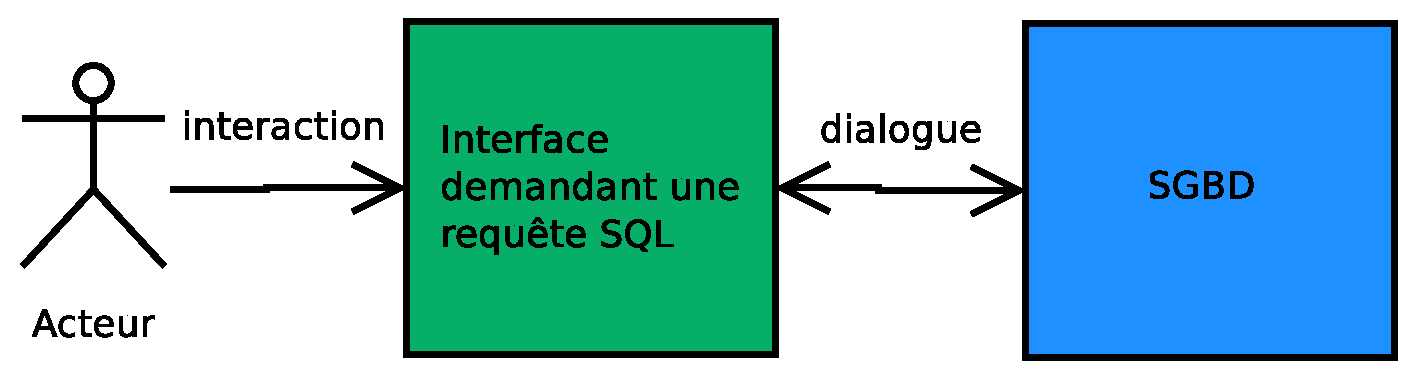
\includegraphics[width=14cm]{images/sans_idb.eps}
  \caption{Utilisation classique d'un SGBD.}
  \label{sans_idb_schema}
\end{figure}

\begin{figure}[!h]
  \centering
  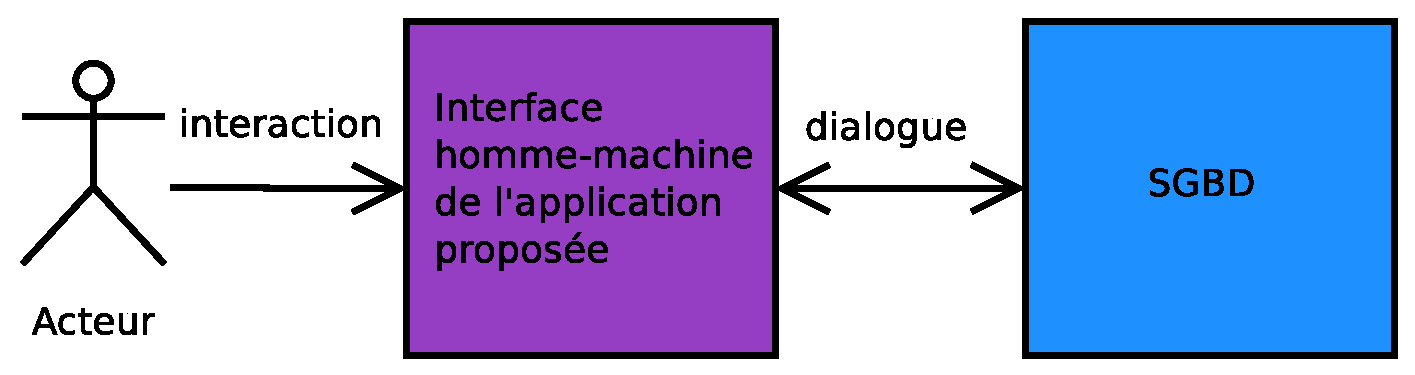
\includegraphics[width=14cm]{images/avec_idb.eps}
  \caption{Utilisation d'un SGBD avec l'application du projet.}
  \label{avec_idb_schema}
\end{figure}

\begin{figure}[!h]
  \centering
  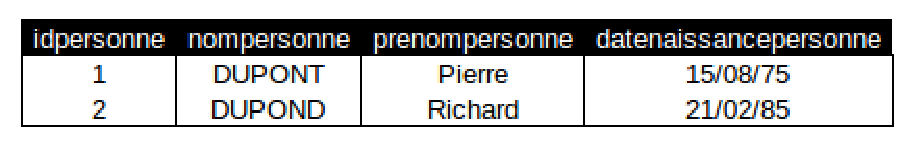
\includegraphics[width=14cm]{images/exemple_table.eps}
  \caption{Un exemple de table avec deux tuples et quatre attributs.}
  \label{exemple_table}
\end{figure}


\backmatter

\end{document}
